\section{Durchführung}
\label{sec:Durchführung}
Die Messung der Temperaturabhängigkeit der Dampfdruckkurve wird in diesem Versuch in zwei verschiedenen Druckbereichen durchgeführt. Im Bereich der negativen
Druckdifferenz wird von $\qty{25}{\milli\bar}$ bis zum Atmosphärendruck von etwa $\qty{1000}{\milli\bar}$ gemessen, während bei einer zweiten Messung im 
Druckbereich von $\qty{1}{\bar}$ bis $\qty{15}{\bar}$ gemessen wird. Für die beiden Druckbereiche wird jeweils ein unterschiedlicher Versuchsaufbau verwendet.

\subsection{Messung im Druckbereich unter Atmosphärendruck}
\label{subsec:D_Unterdruck}
Zur Messung der Dampfdruckkurve im Bereich unter Atmosphärendruck wird der in \autoref{fig:Aufbau1} dargestellte Aufbau verwendet.
\begin{figure}
    \centering
    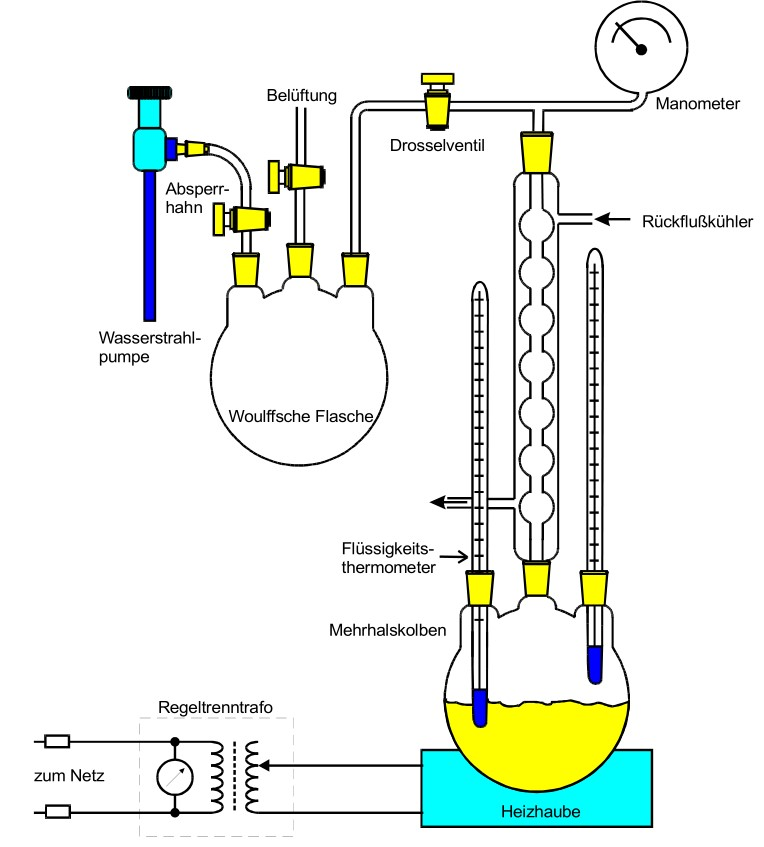
\includegraphics[width =.7\textwidth]{content/Aufbau1.jpg}
    \caption{Skizze zur Messung der Dampfdruckkurve im Bereich von $p \leq \qty{1}{\bar}$ \cite{v203}.}
    \label{fig:Aufbau1}
\end{figure}
Vor Beginn der Messung werden der Atmosphärendruck $p_0$ und die Außentemperatur $T_0$ notiert.
Um die Apparatur zu evakuieren wird die Wasserstrahlpumpe eingeschaltet. Das Drosselventil und der Absperrhahn müssen dabei geöffnet werden, während das 
Belüftungsventil verschlossen bleibt. Auf dem digitalen Druckmessgerät lässt sich der Druck innerhalb der Messaparatur ablesen. Sobald ein Druck von
ca. $\qty{25}{\milli\bar}$ erreicht wird, werden die zuvor geöffneten Ventile verschlossen und die Wasserstrahlpumpe abgestellt. Die Messung kann gestartet werden,
sobald die Kühlwasserzufuhr und die Heizhaube eingeschaltet sind. Während die Temperatur im Inneren des Kolbens steigt, werden Wertepaare von Druck und 
Temperatur zu einer Schrittweite von $\qty{1}{\degreeCelsius}$ notiert. Die Temperatur wird dabei an demjenigen Thermometer abgelesen, welches sich im Dampfraum des 
Kolbens befindet. Bei Erreichen eines Druckes von über $\qty{1000}{\milli\bar}$ wird die Messreihe beendet. Die Heizhaube wird ausgeschaltet. Aus den Messwerten kann
ein Wert für die mittlere Verdampfungswärme im untersuchten Druckbereich bestimmt werden.

\subsection{Messung im Druckbereich über Atmosphärendruck}
\label{subsec:D_Überdruck}
Zur Bestimmung der Temperaturabhängigkeit der Verdampfungswärme wird ein Druckbereich von $\qty{1}{\bar}$ bis $\qty{15}{\bar}$ betrachtet. Der hierzu verwendete Aufbau
kann \autoref{fig:Aufbau2} entnommen werden.

\begin{figure}
    \centering
    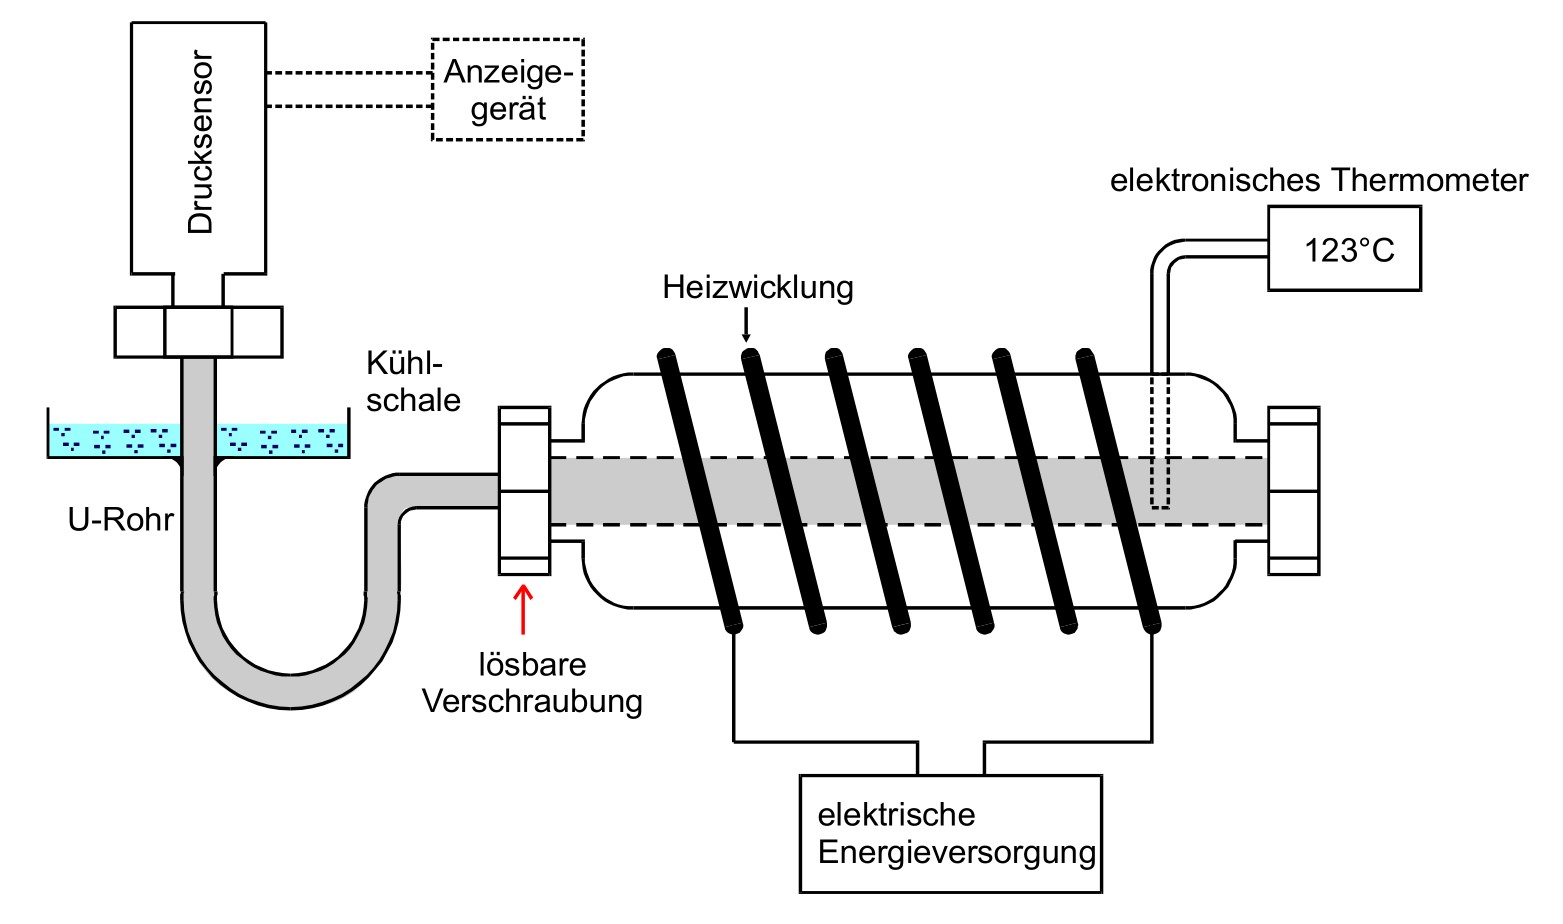
\includegraphics[width =.75\textwidth]{content/Aufbau2.jpg}
    \caption{Skizze zur Messung der Dampfdruckkurve im Bereich von $p \geq \qty{1}{\bar}$ \cite{v203}.}
    \label{fig:Aufbau2}
\end{figure}

Im Hohlraum des abgebildeten Stahlgefäßes befindet sich destilliertes und entgastes Wasser. Dieses wird mithilfe der Heizvorrichtung erhitzt. Zu Beginn der Messung 
sollte die Apparatur auf ca. $\qty{100}{\degreeCelsius}$ vorgeheizt werden. Ist diese Temperatur erreicht, sollte sich die Druckanzeige des Manometers dem Wert von
$\qty{1}{\bar}$ nähern, an welchem die Messreihe begonnen werden kann. Es werden Wertepaare von Druck und Temperatur in Abständen von $\qty{1}{\bar}$ genommen, bis ein 
Druck von $\qty{15}{\bar}$ erreicht wird. 
